\documentclass{beamer}

\usetheme{CambridgeUS}
\usecolortheme{seahorse}

\usepackage{geometry}

\usepackage{algorithm2e}
\usepackage{graphicx}
\usepackage{tabularx}
\usepackage{fourier}
\usepackage{hyperref}
\usepackage{multirow}
\usepackage{caption}
\usepackage{subcaption}
\usepackage{amsmath}
\usepackage{float}





	\usepackage{rotating}	%% introduce sideways env
\usepackage{tikz}
\usepackage{amssymb}

%% Public TikZ libraries
\usetikzlibrary{positioning}
\usetikzlibrary{shapes}
\usetikzlibrary{calc,cipher,sponge}


\usetikzlibrary{arrows}			%% Include regular arrows
\usetikzlibrary{arrows.meta}	
%\usepgflibrary{myarrows.new}		%% Include custom arrows
%\usetikzlibrary{mycrypto.symbols}


\tikzset{XOR/.style={draw,
		circle,
		append after command={
			[shorten >=\pgflinewidth, shorten <=\pgflinewidth,]
			(\tikzlastnode.north) edge[] (\tikzlastnode.south)
			(\tikzlastnode.east) edge[] (\tikzlastnode.west)
		},
	},
}

\tikzset{edge/.style={
		-latex new, 
		arrow head=6pt, 
		%						thick
	},
}

\tikzset{line/.style={
		%						thick,
		draw, 
		%						-latex',
		shorten <=1bp,
		shorten >=1bp,
	}
}

\newcommand{\AEheight}{0.75cm}
\newcommand{\AEwidth}{1.5cm}

\tikzset{AE_P/.style={
		rectangle,
		thick,
		draw,
		fill=yellow!20,
		inner sep = 0pt,
		outer sep = 0pt,
		text width=1cm, 
		minimum height=4.5cm,
		text centered,
		%		anchor=north,
	}	
}

\tikzset{AE_vert/.style={
		rectangle,
		thick,
		draw,
		fill=blue!20,
		inner sep = 0pt,
		outer sep = 0pt,
		text width=\AEheight, 
		minimum height=\AEwidth,
		text centered,
		%		anchor=north,
	}
}

\tikzset{AE_msg/.style={
		rectangle,
		thick,
		draw,
		fill=blue!20,
		inner sep = 0pt,
		outer sep = 0pt,
		text width=\AEwidth,
		minimum height=\AEheight,
		text centered,
		%		anchor=north,
	}
}

\tikzset{AE_ctx/.style={
		rectangle,
		thick,
		draw,
		fill=green!20,
		inner sep = 0pt,
		outer sep = 0pt,
		text width=\AEwidth, 
		minimum height=\AEheight,
		text centered,
		%		anchor=north,
	}
}

\tikzset{AE_key/.style={
		rectangle,
		thick,
		draw,
		fill=red!20,
		inner sep = 0pt,
		outer sep = 0pt,
		text width=\AEwidth, 
		minimum height=\AEheight,
		text centered,
		%		anchor=north,
	}
}

\tikzset{AE_tag/.style={
		rectangle,
		thick,
		draw,
		fill=green!20,
		inner sep = 0pt,
		outer sep = 0pt,
		text width=\AEwidth, 
		minimum height=\AEheight,
		text centered,
		%		anchor=north,
	}
}





\usepackage{xcolor}
\usepackage{listings}

\definecolor{mGreen}{rgb}{0,0.6,0}
\definecolor{mGray}{rgb}{0.5,0.5,0.5}
\definecolor{mPurple}{rgb}{0.58,0,0.82}
\definecolor{backgroundColour}{rgb}{0.95,0.95,0.92}

\lstdefinestyle{CStyle}{
	backgroundcolor=\color{backgroundColour},   
	commentstyle=\color{mGreen},
	keywordstyle=\color{magenta},
	numberstyle=\tiny\color{mGray},
	stringstyle=\color{mPurple},
	basicstyle=\tiny,
	breakatwhitespace=false,         
	breaklines=true,                 
	captionpos=b,                    
	keepspaces=true,                 
	numbers=left,                    
	numbersep=5pt,                  
	showspaces=false,                
	showstringspaces=false,
	showtabs=false,                  
	tabsize=2,
	language=C
}

\setbeamertemplate{navigation symbols}{}

\author{Alexane Boldo}

\institute[]{ENS Rennes \and
		OCIF, IRISA \and
		IMT Atlantique}

\title{Side-channel attacks on Ascon's S-box}

\date{May-July 2025}

\setbeamertemplate{page number in head/foot}[appendixframenumber]

\begin{document}
	\begin{frame}
		\maketitle\small
		{\centering\itshape Supervisor: Hélène Le Bouder\par}
	\end{frame}
	
	\begin{frame}
		\frametitle{Introduction}
		\textbf{Side-Channel Attacks (SCA):} observation of computation time, power consumption, electromagnetic radiation, ... to discover a secret
		
		$\newline$
		
		\textbf{Goal:} Study the leaks from the winner for lightweight cryptography Ascon to theorize a SCA attack
	\end{frame}
	
%	\AtBeginSection[]
%	{
%		\begin{frame}
%			\frametitle{Table of Contents}
%			\tableofcontents[currentsection]
%		\end{frame}
%	}
	
	\begin{frame}
		\frametitle{Table of Contents}
		\tableofcontents
	\end{frame}
	
	\section{Ascon-AEAD}
	\subsection{Presentation}
	\begin{frame}
		\frametitle{What is Ascon-AEAD?}
		\textbf{Authenticated Encryption with Associated Data (AEAD)}: encrypt, check authentication of content and associated data
		
		\begin{figure}
			\centering
			\begin{tikzpicture}[node distance = 1cm]

\node[AE_msg] (aead) {AEAD};

\node[left = of $(aead.north west)!3/4!(aead.south west)$] (m) {$M$};
\node[left = of $(aead.north west)!1/4!(aead.south west)$] (a) {$A$};

\node[above = of $(aead.north west)!1/4!(aead.north east)$] (k) {$K$};
\node[above = of $(aead.north west)!3/4!(aead.north east)$] (n) {$N$};

\node[right = of $(aead.north east)!1/4!(aead.south east)$] (c) {$C$};
\node[right = of $(aead.north east)!3/4!(aead.south east)$] (t) {$T$};


\draw[-{Latex[length=2mm]}] (m) -- (aead.west|-m);
\draw[-{Latex[length=2mm]}] (a) -- (aead.west|-a);

\draw[-{Latex[length=2mm]}] (k) -- (aead.north-|k);
\draw[-{Latex[length=2mm]}] (n) -- (aead.north-|n);

\draw[-{Latex[length=2mm]}] (aead.east|-c) -- (c);
\draw[-{Latex[length=2mm]}] (aead.east|-t) -- (t);

\end{tikzpicture}
			\caption{AEAD algorithm from \cite{cours_crypto}}
		\end{figure}
		
	\end{frame}
	
	\begin{frame}
		\frametitle{Ascon's State}
		\begin{tabular}{ccccccccl}
			byte 0&byte 1&byte 2&byte 3&byte 4&byte 5&byte 6&byte 7&\\
			\cline{1-8}
			\multicolumn{8}{|c|}{IV}&$S_0$\\
			\cline{1-8}
			\multicolumn{8}{|c|}{first half of K, $K_0$}&$S_1$\\
			\cline{1-8}
			\multicolumn{8}{|c|}{second half of K, $K_1$}&$S_2$\\
			\cline{1-8}
			\multicolumn{8}{|c|}{first half of N, $N_0$}&$S_3$\\
			\cline{1-8}
			\multicolumn{8}{|c|}{second half of N, $N_1$}&$S_4$\\
			\cline{1-8}
		\end{tabular}
	\end{frame}
	
	\subsection{Encryption and decryption phases}
	\begin{frame}
		\frametitle{Encryption and decryption phases}
		
		4 phases: initialization, associated data process, plaintext/ciphertext process, finalization
		
		\begin{figure}
			\centering
			\resizebox{350pt}{80pt}{
				\resizebox{250pt}{50pt}{
	
\begin{tikzpicture}[node distance = 1cm and 0.75cm]

% init
\node[AE_P, minimum height = 3.75cm] (pi) {$p^{12}$};

\node[AE_vert, fill = gray!20, left = of pi.north west, anchor = north east, minimum height = 0.75cm] (iv) {$IV$}; 

\node[AE_vert, fill = red!20, anchor = north] (k)  at (iv.south) {$K$}; 
\node[AE_vert, fill = blue!20, left = of pi.south west, anchor = south east] (n) {$N$}; 

\coordinate (helpsouth) at ($(pi.south east)!1/6!(pi.north east)$);
\coordinate (helpnorth) at ($(pi.south east)!5/6!(pi.north east)$);

\draw[-{Latex[length=2mm]}] (iv.east|-helpnorth) -> (helpnorth-|pi.west) node[midway] {$/$} node[midway, below=0.2cm] {\small $64$};
\draw[-{Latex[length=2mm]}] (k.east|-pi.west) -- (pi.west) node[midway] {$/$} node[midway, below=0.2cm] {\small $128$};
\draw[-{Latex[length=2mm]}] (n.east|-helpsouth) -- (helpsouth-|pi.west) node[midway] {$/$} node[midway, below=0.2cm] {\small $128$};

\node[XOR, right = of pi.east|-helpsouth] (xkinit) {};
\node[AE_key, anchor = west, below = of xkinit, path picture={
      \fill[gray!20] (path picture bounding box.north) rectangle (path picture bounding box.south west);
    }] (kinit) {$0^* || K$};

\draw[-{Latex[length=2mm]}] (pi.east|-helpsouth) -- (xkinit) node[midway] {$/$} node[midway, below=0.2cm] {\small $256$}; 
\draw[-{Latex[length=2mm]}] (kinit.north-|xkinit) -- (xkinit); 



% 1er tour AD

\node[XOR, right = of kinit.east|-helpnorth] (xa1) {};

\node[AE_msg, above = of xa1] (a1) {$A_1$};

\draw[-{Latex[length=2mm]}] (a1) -- (xa1) node[midway] {$/$} node[midway, left=0.2cm] {\small $64$};
\draw[line] (pi.east|-xa1) -- (helpnorth-|xkinit) node[midway] {$/$} node[midway, below=0.2cm] {\small $64$};
\draw[-{Latex[length=2mm]}] (pi.east|-xa1)  -- (xa1);


% 2er tour AD


\node[AE_P, minimum height = 3.75cm, right = of xa1|-pi] (pa1) {$p^{8}$};

\draw[-{Latex[length=2mm]}] (xkinit) -- (pa1.west|-xkinit);
\draw[-{Latex[length=2mm]}] (xa1) -- (pa1.west|-xa1);

\node[right = of pa1.east|-helpnorth, inner sep = 10pt] (cdotnortha) {$\cdots$};
\node[right = of pa1.east|-helpsouth, inner sep = 10pt] (cdotsoutha) {$\cdots$};

\node[XOR, right = of cdotnortha] (xa2) {};
\node[AE_msg, above = of xa2, path picture={
      \fill[gray!20] (path picture bounding box.north) rectangle (path picture bounding box.south east);
    }] (a2) {$A_{s}||10^*$};


\draw[line] (pa1.east|-cdotnortha) -- (cdotnortha);
\draw[line] (pa1.east|-cdotsoutha) -- (cdotsoutha);
\draw[-{Latex[length=2mm]}] (cdotnortha) -- (xa2);
\draw[-{Latex[length=2mm]}] (a2) -- (xa2) node[midway] {$/$} node[midway, left=0.2cm] {\small $64$};


% fin AD

\node[AE_P, minimum height = 3.75cm, right = of xa2|-pa1] (pa2) {$p^{8}$};

\node[XOR, right = of pa2.east|-helpsouth] (xdom) {};
\node[AE_key, fill = gray!20, below = of xdom] (dom) {$0^*1$};

\draw[-{Latex[length=2mm]}] (xa2) -- (pa2.west|-xa2);
\draw[-{Latex[length=2mm]}] (cdotsoutha) -- (pa2.west|-helpsouth);

\draw[-{Latex[length=2mm]}] (pa2.east|-xdom) -- (xdom);
\draw[-{Latex[length=2mm]}] (dom.north-|xdom) -- (xdom);



% 1er tour chiffrement

\node[XOR, right = of dom.east|-helpnorth] (x1) {};
\node[AE_msg, above = of x1] (m1) {$M_1$};
\node[AE_ctx, right = of m1] (c1) {$C_1$};

\draw[-{Latex[length=2mm]}] (pa2.east|-x1) -- (x1);
\draw[-{Latex[length=2mm]}] (m1) -- (x1) node[midway] {$/$} node[midway, left=0.2cm] {\small $64$};
\draw[-{Latex[length=2mm]}] (x1) -| (c1)node[near end] {$/$} node[near end, left=0.2cm] {\small $64$};

\node at (x1-|c1) {$\bullet$};

% 2e tour chiffrement

\node[AE_P, minimum height = 3.75cm, right = of c1|-pa2] (p1) {$p^{8}$};

\draw[-{Latex[length=2mm]}] (x1) -- (x1-|p1.west);
\draw[-{Latex[length=2mm]}] (xdom) -- (p1.west|-helpsouth);

\node[right = of p1.east|-helpnorth, inner sep = 10pt] (cdotnorth) {$\cdots$};
\node[right = of p1.east|-helpsouth, inner sep = 10pt] (cdotsouth) {$\cdots$};

\node[XOR, right = of cdotnorth] (x2) {};
\node[AE_msg, above = of x2] (m2) {$M_{t-1}$};
\node[AE_ctx, right = of m2] (c2) {$C_{t-1}$};


\draw[line] (p1.east|-cdotnorth) -- (cdotnorth);
\draw[line] (p1.east|-cdotsouth) -- (cdotsouth);

\draw[-{Latex[length=2mm]}] (cdotnorth) -- (x2);
\draw[-{Latex[length=2mm]}] (m2) -- (x2) node[midway] {$/$} node[midway, left=0.2cm] {\small $64$};
\draw[-{Latex[length=2mm]}] (x2) -| (c2) node[near end] {$/$} node[near end, left=0.2cm] {\small $64$};

\node at (x2-|c2) {$\bullet$};


% fin chiffrement

\node[AE_P, minimum height = 3.75cm, right = of c2|-p1] (p2) {$p^{8}$};

\draw[-{Latex[length=2mm]}] (x2) -- (x2-|p2.west);
\draw[-{Latex[length=2mm]}] (cdotsouth) -- (p2.west|-cdotsouth);

\node[XOR, right = of p2.east|-x1] (x3) {};
\node[AE_msg, above = of x3, path picture={
      \fill[gray!20] (path picture bounding box.north) rectangle (path picture bounding box.south east);
    }] (m3) {$M_{t}||10^*$};
\node[AE_ctx, right = of m3, text width = 0.75cm] (c3) {$C_{t}$};

\draw[-{Latex[length=2mm]}] (p2.east|-x3) -- (x3);
\draw[-{Latex[length=2mm]}] (m3) -- (x3) node[midway] {$/$} node[midway, left=0.2cm] {\small $64$};
\draw[-{Latex[length=2mm]}] (x3) -| (c3) node[near end] {$/$} node[near end, left=0.2cm] {\small $|M_t|$};

\node at (x3-|c3) {$\bullet$};


% finalisation

\node[XOR, right = of c3.east|-helpsouth] (xkf) {};

\node[AE_P, minimum height = 3.75cm, right = of xkf.east|-p2] (pf) {$p^{12}$};

\node[AE_key, below = of xkf, path picture={
      \fill[gray!20] (path picture bounding box.north) rectangle (path picture bounding box.south east);
    }] (kf) {$K||0^*$};

\draw[-{Latex[length=2mm]}] (x3) -- (x3-|pf.west);
\draw[-{Latex[length=2mm]}] (p2.east|-xkf) -- (xkf);
\draw[-{Latex[length=2mm]}] (xkf|-kf.north) -- (xkf);
\draw[-{Latex[length=2mm]}] (xkf) -- (xkf-|pf.west);

\node[XOR, right = of pf.east|-xkf] (xt) {};
\node[AE_key, below = of xt] (kt) {$K$};
\node[AE_tag] at (c3-|xt) (t) {$T$};

\draw[-{Latex[length=2mm]}] (pf.east|-xt) -- (xt) node[midway] {$/$} node[midway, below=0.2cm] {\small $128$};
\draw[-{Latex[length=2mm]}] (kt) -- (xt);
\draw[-{Latex[length=2mm]}] (xt) -- (t);


% separations

\coordinate (sepinit) at ($(kinit.east)!1/2!(a1.west)$);
\draw[line, dashed] (kinit.south-|sepinit) -- (a1.north-|sepinit);

\coordinate (sepa) at ($(dom.east)!1/2!(m1.west)$);
\draw[line, dashed] (dom.south-|sepa) -- (m1.north-|sepa);

\coordinate (sepf) at ($(c3.east)!1/2!(kf.west)$);
\draw[line, dashed] (kf.south-|sepf) -- (c3.north-|sepf);

\end{tikzpicture}
}
			}
			\caption{Ascon-AEAD mode, from \cite{cours_crypto}}
		\end{figure}	
	\end{frame}
	
	\subsection{The permutation}
	\begin{frame}
		\frametitle{Ascon's permutation}
		
		\begin{columns}
			\column{0.47\textwidth}
			$p = p_L \circ \underbrace{p_S}{} \circ p_C$\\
			\begin{figure}
				\resizebox*{150pt}{90pt}{
					\newcommand{\advanceS}[1][.5]{\draw (s) + (#1,0) coordinate (s);}
\newcommand{\updateTo}[2]{ \draw[next] (#1) -- (#2); \node also [alias=#1] (#2); }
\begin{tikzpicture}[scale=.70, rounded corners=2pt,
	op/.append style={minimum size=1.25ex},
	tee/.style={}, every node/.append style={inner sep=1pt}]
	% --- inputs ---
	\coordinate (s);
	\foreach \x in {0,...,5} { \draw (s|-0,-\x) coordinate (w\x); }
	\node[left] (x0) at (w0) {$IV$};
	\node[left] (x1) at (w1) {$K_0$};
	\node[left] (x2) at (w2) {$K_1$};
	\node[left] (x3) at (w3) {$N_0$};
	\node[left] (x4) at (w4) {$N_1$};
	
	% --- input xors ---
	\advanceS
	\draw (s|-w0) coordinate[xor] (in0);  \updateTo{w0}{in0}
	\draw (s|-w4) coordinate[tee] (tin0); \draw[next] (tin0) -- (in0);
	\advanceS
	\draw (s|-w2) coordinate[xor] (in2);  \updateTo{w2}{in2}
	\draw (s|-w1) coordinate[tee] (tin2); \draw[next] (tin2) -- (in2);
	\draw (s|-w4) coordinate[xor] (in4);  \updateTo{w4}{in4}
	\draw (s|-w3) coordinate[tee] (tin4); \draw[next] (tin4) -- (in4);
	
	% --- chi nots ---
	\advanceS
	\draw (s|-w0) coordinate[tee] (tand4);
	\advanceS
	\foreach \x in {0,...,4} { \draw (s|-w\x) +(0,-.5) node[left] (cnot\x) {$1$}; }
	\advanceS
	\foreach \x in {0,...,4} { \draw (s|-w\x)    coordinate[tee] (tnot\x);
		\draw (s|-cnot\x) coordinate[xor] (not\x);
		\draw[next] (cnot\x) -- (not\x);
		\draw[next] (tnot\x) -- (not\x); }
	
	% --- chi ands ---
	\advanceS[.75]
	\foreach \x in {0,...,4} { \draw (s|-cnot\x) coordinate[andalt] (and\x);
		\draw[next] (not\x) -- (and\x); }
	\foreach \x/\X in {0/1,1/2,2/3,3/4} { \draw (and\x|-w\X) coordinate[tee] (tand\x); 
		\draw[next] (tand\x) -- (and\x); }
	\draw[next] (tand4) |- (not4|-w5) -| (and4);
	
	% --- chi xors ---
	\advanceS[1.25]
	\foreach \x in {0,...,4} { \draw (s|-w\x) coordinate[xor] (xor\x);
		\updateTo{w\x}{xor\x} }
	\foreach \x/\X in {0/1,1/2,2/3,3/4} { \draw[next] (and\X) -- +(.3,0) -- (xor\x|-and\x) -- (xor\x); }
	\draw[next] (and0) -- +(.3,0) -- ($(and4)!.5!(xor4|-and4)$) -- (xor4|-and4) -- (xor4);
	
	% --- output xors ---
	\advanceS[.75]
	\draw (s|-w1) coordinate[xor] (out1);  \updateTo{w1}{out1}
	\draw (s|-w0) coordinate[tee] (tout1); \draw[next] (tout1) -- (out1);
	\draw (s|-w3) coordinate[xor] (out3);  \updateTo{w3}{out3}
	\draw (s|-w2) coordinate[tee] (tout3); \draw[next] (tout3) -- (out3);
	\advanceS
	\draw (s|-w0) coordinate[xor] (out0);  \updateTo{w0}{out0}
	\draw (s|-w4) coordinate[tee] (tout0); \draw[next] (tout0) -- (out0);
	\advanceS
	\draw (s|-w2) coordinate[xor] (out2);  \updateTo{w2}{out2}
	\draw (s|-and2) node[below] (cout2) {$1$};
	\draw[next] (cout2) -- (out2);
	%\draw (s|-and2) node[left=.15] (cout2) {$1$};
	%\draw[next] (cout2) -| (out2);
	
	% --- outputs ---
	\advanceS
	\foreach \x in {0,...,4} { \node[right] (y\x) at (s|-w\x) {$out_{\x}$}; \updateTo{w\x}{y\x} }
\end{tikzpicture}
				}
				\caption{Circuit to compute the S-box, from \cite{crypto_schema}, permutation of $\llbracket1;31 \rrbracket$}
				\label{circuit_sbox}
			\end{figure}
			
			\column{0.47\textwidth}
			\begin{figure}[h]
				\centering
				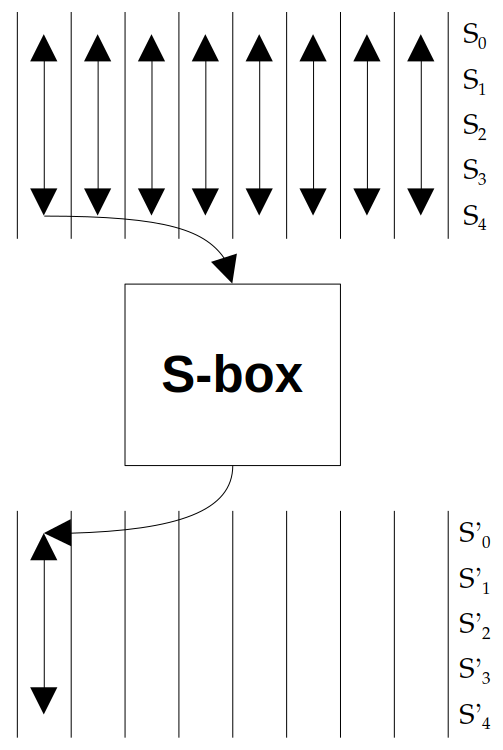
\includegraphics[width=0.6\linewidth]{img_files/sbox_illustration}
				\caption{S-box computation for the first byte of each word}
				\label{fig:comp}
			\end{figure}

		\end{columns}
	\end{frame}
	
	\subsection{An analysis of the S-box}
	\begin{frame}
		\frametitle{Table linking the output of the S-box and the key}
		\begin{figure}[h]
			\centering
			\begin{tabular}{|c|c|}
				\hline
				$(N_0^j,N_1^j,IV^j)$&$S_4^j$\\
				\hline\hline
				$(0,0,0)$&$K_0^j$\\
				\hline
				$(0,0,1)$&$0$\\
				\hline
				$(0,1,0)$&$1$\\
				\hline
				$(0,1,1)$&$1 \oplus K_0^j$\\
				\hline
				$(1,0,0)$&$1 \oplus K_0^j$\\
				\hline
				$(1,0,1)$&$1$\\
				\hline
				$(1,1,0)$&$0$\\
				\hline
				$(1,1,1)$&$K_0^j$\\
				\hline
			\end{tabular}
			\caption{Link between $K_0^j$ and $S_4^j$ depending on $IV$ and $N$, from \cite{these}}
			\label{link_k_s4}
		\end{figure}
	\end{frame}
	
	\section{A side-channel attack}
	\subsection{Hardware}
	\begin{frame}
		\frametitle{ChipWhisperer-Lite}
		\begin{figure}[h]
			\raggedright
			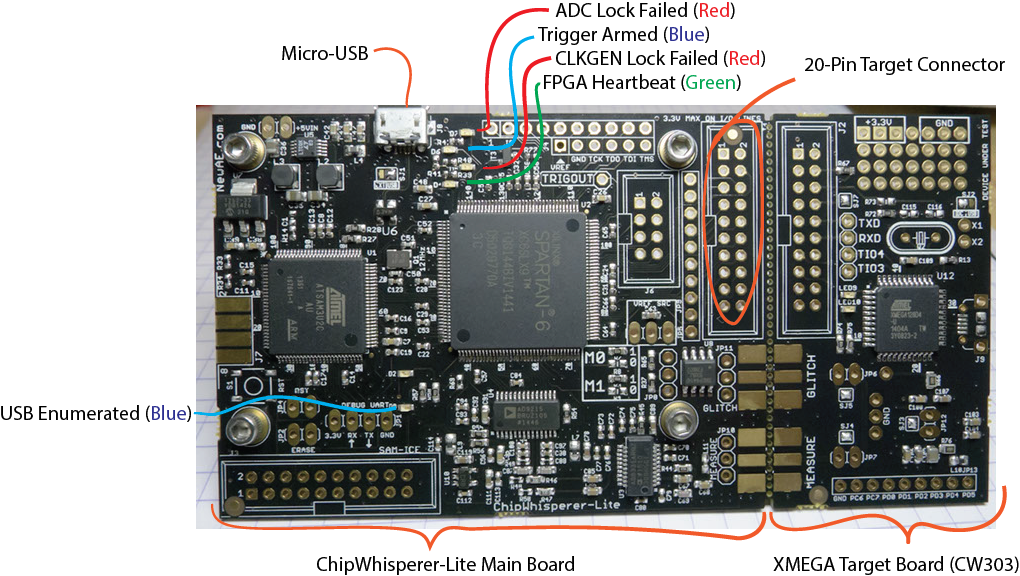
\includegraphics[width=0.9\textwidth]{img_files/cwlite_basic1}
			\caption{ChipWhisperer Lite board, from \cite{cwdoc}}
			\label{fig:cw}
		\end{figure}
	\end{frame}

	\subsection{Analysis}
	\begin{frame}
		\frametitle{Analyses done}
		\begin{figure}
			\centering
			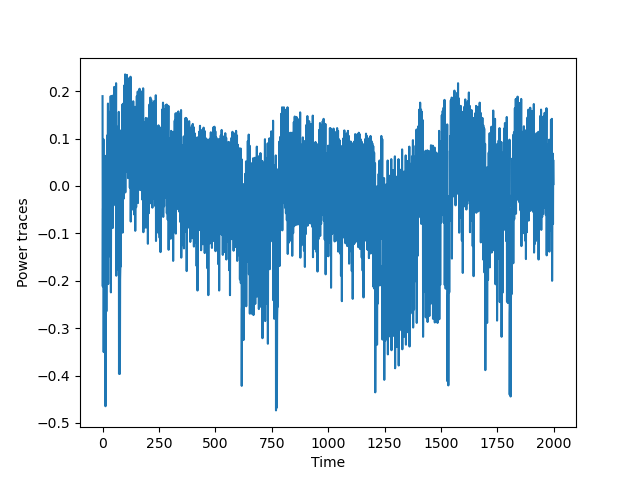
\includegraphics[width=0.5\textwidth]{img_files/trace_ascon}
			\caption{Power trace during Ascon's S-box}
		\end{figure}
		\begin{itemize}
			\item{Finding the best model}
				\begin{itemize}
					\item{Vertical vs horizontal}
					\item{HW vs value}
				\end{itemize}
			\item{Attack: finding the vertical output and deduce the key}
		\end{itemize}
	\end{frame}
	
	
	\section{Results}
	\begin{frame}
		\frametitle{Results vertical vs horizontal and HW vs value}
		\begin{columns}[T]
			\column{0.47\textwidth}
			\begin{figure}[h]
				\centering
				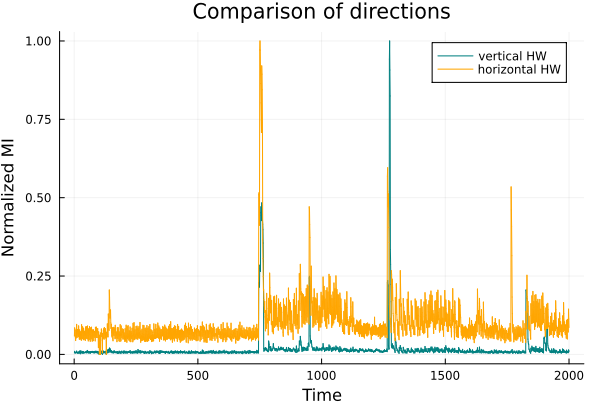
\includegraphics[scale=0.25]{img_files/h_and_v_one_byte}
				\caption{Mutual information for the horizontal and the vertical value}
				\label{hvval}
			\end{figure}
			\column{0.47\textwidth}
			\begin{figure}
				\centering
				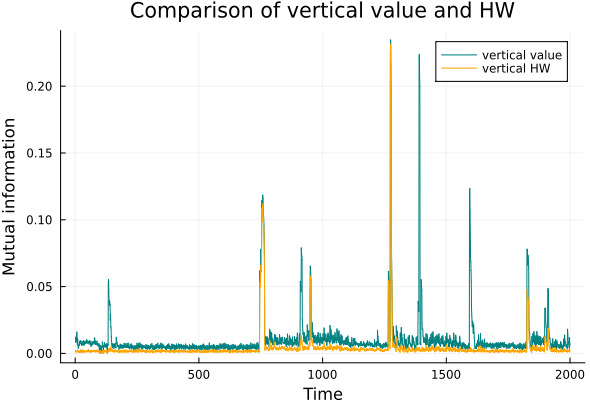
\includegraphics[scale=0.25]{img_files/vertical_one_bit}
				\caption{Mutual information between power consumption and HW or value}
				\label{vHW}
			\end{figure}
		\end{columns}
	\end{frame}
	
%	\begin{frame}
%		\frametitle{Results distinguisher}
%		\begin{figure}
%			\centering
%			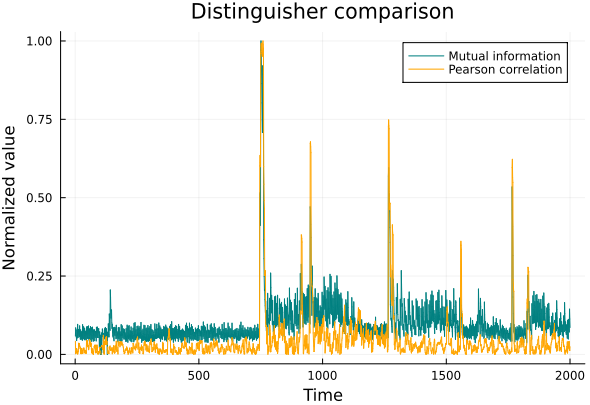
\includegraphics[scale=0.3]{img_files/corr_vs_MI_hHW}
%			\caption{Mutual information and absolute Pearson correlation for a horizontal attack on the reference implementation}
%			\label{corvsMI}
%		\end{figure}
%	\end{frame}
	
	\begin{frame}
		\frametitle{Results attack}
		\begin{figure}[h]
			\centering
			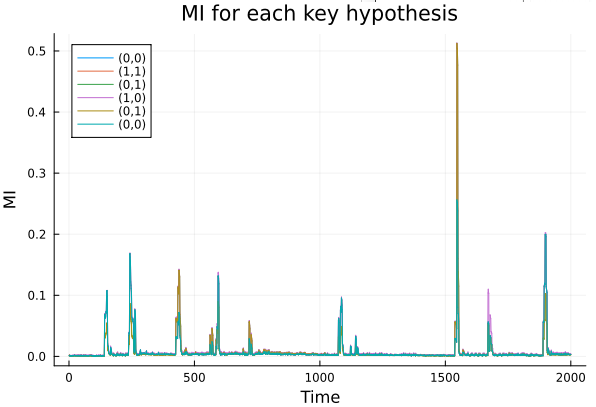
\includegraphics[scale=0.3]{img_files/nonces_alea}
			\caption{Mutual information between the HW of the outputs and the power consumption, for each of the possible outputs for the first nonce}
			\label{all_alea}
		\end{figure}
	\end{frame}
	
	\section{Conclusion}
	\begin{frame}
		\frametitle{Conclusion}
		\begin{itemize}
			\item Good leaks compared to random values
			\item Though apparent weaknesses, unsuccessful attempts
			\item Not enough randomness with false key hypotheses
			\item Leads to follow: belief propagation
		\end{itemize}
	\end{frame}
	
	
	\appendix
	\bibliographystyle{IEEEtran} 
	\bibliography{IEEEabrv,refs}
	
	
	\section{Complements for the permutation}
	\begin{frame}
		\frametitle{Permutation (1), $p_C$}
		
		Constant for the round $i$: $const_{16-nb_{rounds}+i}$\\
		
		\begin{figure}[h]
				\centering
				\footnotesize
				\begin{tabularx}{0.5\textwidth}{cc||cc}
					\hline
					$i$&\verb|const|$_i$&$i$&\verb|const|$_i$\\
					\hline
					0&\verb|0x000000000000003c|&8&\verb|0x00000000000000b4|\\
					1&\verb|0x000000000000002d|&9&\verb|0x00000000000000a5|\\
					2&\verb|0x000000000000001e|&10&\verb|0x0000000000000096|\\
					3&\verb|0x000000000000000f|&11&\verb|0x0000000000000087|\\
					4&\verb|0x00000000000000f0|&12&\verb|0x0000000000000078|\\
					5&\verb|0x00000000000000e1|&13&\verb|0x0000000000000069|\\
					6&\verb|0x00000000000000d2|&14&\verb|0x000000000000005a|\\
					7&\verb|0x00000000000000c1|&15&\verb|0x000000000000004b|\\
					\hline
				\end{tabularx}
				\caption{Constant-addition layer, constants}
				\label{consts}
			\end{figure} 
		\end{frame}
		
		\begin{frame}
			\frametitle{Permutation (2), $p_C$}
			\begin{figure}[h]
				\centering
				\begin{tabularx}{0.4\textwidth}{|*{8}{>{\centering\arraybackslash}X|}>{\centering\arraybackslash}X}
					\cline{1-8}
					&&&&&&&&$S_0$\\
					\cline{1-8}
					&&&&&&&&$S_1$\\
					\cline{1-8}
					&&&&&&& \LARGE $\oplus$&$S_2$\\
					\cline{1-8}
					&&&&&&&&$S_3$\\
					\cline{1-8}
					&&&&&&&&$S_4$\\
					\cline{1-8}
				\end{tabularx}
				\caption{Constant-addition layer, each box representing a byte of one of the 64-bit words}
				\label{const_lay}
			\end{figure}
	\end{frame}
		
	
		
	\begin{frame}
		\frametitle{Permutation (3), $p_S$}
		
			\begin{figure}[h]
				\small
				\centering
				\begin{tabular}{|c||*{8}{c|}}
					\hline
					$x$&0&1&2&3&4&5&6&7\\
					\hline
					$S-box(x)$&4&b&1f&14&1a&15&9&2\\
					\hline\hline
					$x$&8&9&a&b&c&d&e&f\\
					\hline
					$S-box(x)$&1b&5&8&12&1d&3&6&1c\\
					\hline\hline
					$x$&10&11&12&13&14&15&16&17\\
					\hline
					$S-box(x)$&1e&13&7&e&0&d&11&18\\
					\hline\hline
					$x$&18&19&1a&1b&1c&1d&1e&1f\\
					\hline
					$S-box(x)$&10&c&1&19&16&a&f&17\\
					\hline
				\end{tabular}
				\caption{Lookup table for the 5-bit S-box}
				\label{lookup_sbox}
			\end{figure}
	\end{frame}
		
	\begin{frame}[fragile]	
	\frametitle{Permutation (4), $p_S$}
			\begin{figure}[H]
				\begin{lstlisting}[style=CStyle]
					state[0] ^= state[4];
					state[4] ^= state[3];
					state[2] ^= state[1];
					uint64_t t0 = ~state[0];
					uint64_t t1 = ~state[1];
					uint64_t t2 = ~state[2];
					uint64_t t3 = ~state[3];
					uint64_t t4 = ~state[4];
					t0 &= state[1];
					t1 &= state[2];
					t2 &= state[3];
					t3 &= state[4];
					t4 &= state[0];
					state[0] ^= t1
					; state[1] ^= t2;
					state[2] ^= t3;
					state[3] ^= t4;
					state[4] ^= t0;
					state[1] ^= state[0];
					state[0] ^= state[4];
					state[3] ^= state[2];
					state[2] =~ state[2];
				\end{lstlisting}
				\caption{Equations to compute the S-box}
				\label{equations_sbox}
			\end{figure}
			
	\end{frame}
		
	\begin{frame}
		\frametitle{Permutation (5), $p_L$}
		Diffusion: $S_i \leftarrow \Sigma_i(S_i)$:
		
		\begin{gather*}
			\Sigma_0(S_0) = S_0 \oplus (S_0 >>> 19) \oplus (S_0 >>> 28)\\
			\Sigma_1(S_1) = S_1 \oplus (S_1 >>> 61) \oplus (S_1 >>> 39)\\
			\Sigma_2(S_2) = S_2 \oplus (S_2 >>> \;  1) \oplus (S_2 >>> \; 6)\\
			\Sigma_3(S_3) = S_3 \oplus (S_3 >>> 10) \oplus (S_3 >>> 17)\\
			\Sigma_4(S_4) = S_4 \oplus (S_4 >>> \; 7) \oplus (S_4 >>> 41)\\
		\end{gather*}
	\end{frame}		
	
	
	\section{Equations for linking the output of the S-box to the key}
	\begin{frame}
		\frametitle{Finding this table (1)}
		\begin{gather*}
			S_4^j = n_o^j \oplus n_1^j \oplus k_0^j \times (1 \oplus IV^j \oplus n_1^j)\\
			S _4^j =\left \{	
			\begin{array}{ll}
				k_0^j \times (1 \oplus IV^j) & if\ (n_0^j,n_1^j)=(0,0)\\
				k_0^j \times IV^j & if\ (n_0^j,n_1^j)=(1,1)\\
				1 \oplus k_0^j \times IV^j & if\ (n_0^j,n_1^j)=(0,1)\\
				1 \oplus k_0^j \times (1 \oplus IV^j) & if\ (n_0^j,n_1^j)=(1,0)\\
			\end{array}
			\right.
		\end{gather*}
	\end{frame}
	
	\begin{frame}
		\frametitle{Finding this table (2)}
		\noindent Then if $IV^j = 0$: 
		$$S _4^j =\left \{	
		\begin{array}{ll}
			k_0^j& if\ (n_0^j,n_1^j)=(0,0)\\
			0& if\ (n_0^j,n_1^j)=(1,1)\\
			1& if\ (n_0^j,n_1^j)=(0,1)\\
			1 \oplus k_0^j& if\ (n_0^j,n_1^j)=(1,0)\\
		\end{array}
		\right.$$
	\end{frame}
	
	\begin{frame}
		\frametitle{Finding this table (3)}
		\noindent Otherwise, if $IV^j = 1$:
		$$S _4^j =\left \{	
		\begin{array}{ll}
			0& if\ (n_0^j,n_1^j)=(0,0)\\
			k_0^j& if\ (n_0^j,n_1^j)=(1,1)\\
			1 \oplus k_0^j& if\ (n_0^j,n_1^j)=(0,1)\\
			1& if\ (n_0^j,n_1^j)=(1,0)\\
		\end{array}
		\right.$$
	\end{frame}
	
	\section{Complementary graphs}
	\begin{frame}
		\frametitle{Complementary graph (1)}
		\begin{figure}[H]
			\centering
			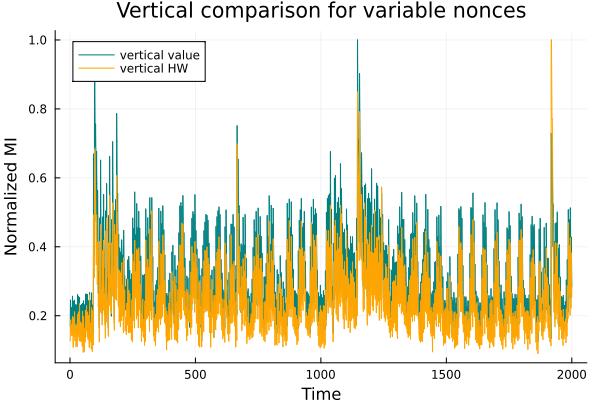
\includegraphics[scale=0.3]{img_files/vertical_one_byte}
			\caption{Mutual information between power consumption and Hamming weight of the concatenation of the first bit of each of the word of $S$ and its value like \ref{vHW} but for random nonces}
			\label{vHW&val}
		\end{figure}
	\end{frame}
	
	\begin{frame}
		\frametitle{Complementary graph (2)}
		\begin{figure}[H]
			\centering
			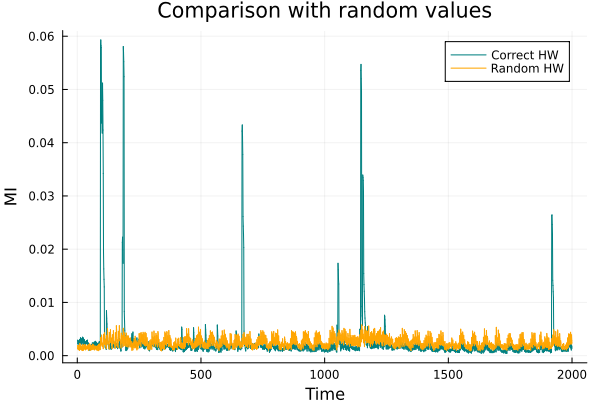
\includegraphics[scale=0.3]{img_files/HWalea}
			\caption{Mutual information between power consumption and vertical HW or random possible HW}
			\label{HWalea}
		\end{figure}
	\end{frame}
	
	\section{Main code} \lstinputlisting[language=C,style=Cstyle,caption=Implementation for ascon.c]{code_files/ascon.c}
	
	\lstinputlisting[language=C,style=Cstyle,caption=Implementation for ascon.h]{code_files/ascon.h}
	
	\lstinputlisting[language=C,style=Cstyle,caption=Implementation for permutation.c]{code_files/permutation.c}
	
	\lstinputlisting[language=C,style=Cstyle,caption=Implementation for permutation.h]{code_files/permutation.h}
	
	\lstinputlisting[language=C,style=Cstyle,caption=Implementation for main.c]{code_files/main.c}
	
	\lstinputlisting[language=Python,style=Cstyle,caption=Implementation for trace capture for the ChipWhisperer]{code_files/traces_sca.py}
	
	\lstinputlisting[style=CStyle, caption=Analysis in Julia of the traces following the established attack]{code_files/decryption_analysis_cpa.jl}
	

\end{document}